\documentclass{article}
\usepackage{amsmath,amsthm,graphicx,hyperref,siunitx}
\newtheorem{theorem}{Theorem}
\newtheorem{lemma}{Lemma}
\newcommand{\ket}[1]{\left|#1\right\rangle}

\title{A derivation written in LaTeX}
\author{Siavash Davani}
\date{2026}

\begin{document}
\maketitle

\begin{abstract}
This page is a plain \texttt{.tex} file. It is parsed by MyST and rendered by Astro.
\end{abstract}

\section{Wave equation}\label{sec:wave}

Starting from Eq.~\eqref{eq-schrodinger} on the theory page and the signal in Figure~\ref{fig-signal},
we write a wave packet as
\begin{equation}
  \psi(x,t) = \int \phi(k)\, e^{i(kx - \omega(k) t)}\, \mathrm{d}k .
  \label{eq:packet}
\end{equation}
Its group and phase velocities follow from Eq.~\eqref{eq:packet}; MyST numbers the whole \texttt{align} block once:
\begin{align}
  v_g &= \frac{\partial \omega}{\partial k} \label{eq:vg} \\
  v_p &= \frac{\omega}{k} . \label{eq:vp}
\end{align}

\begin{theorem}\label{thm:ehrenfest}
Expectation values obey the classical equations of motion, $\frac{d}{dt}\langle x\rangle = \langle p\rangle/m$.
\end{theorem}

\begin{lemma}\label{lem:norm}
The norm $\langle\psi|\psi\rangle$ is conserved.
\end{lemma}

\subsection{A figure and a table}\label{sec:figtab}

\begin{figure}[h]
  \centering
  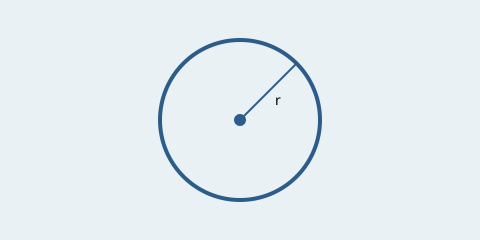
\includegraphics[width=0.5\textwidth]{images/orbit.svg}
  \caption{The orbit again, now included from a LaTeX source.}
  \label{fig:tex-orbit}
\end{figure}

\begin{table}[h]
  \centering
  \caption{Constants used.}
  \label{tab:constants}
  \begin{tabular}{lr}
    \hline
    Quantity & Value \\
    \hline
    $\hbar$ & \SI{1.0546e-34}{\joule\second} \\
    $m_e$ & \SI{9.109e-31}{\kilo\gram} \\
    \hline
  \end{tabular}
\end{table}

Figure~\ref{fig:tex-orbit}, Table~\ref{tab:constants}, Theorem~\ref{thm:ehrenfest} and
Lemma~\ref{lem:norm} are numbered automatically; see also Section~\ref{sec:wave}.
We follow \cite{nielsen2010} and \citet{schrodinger1926}.\footnote{A footnote, numbered by MyST.}

\begin{itemize}
  \item \textbf{bold}, \emph{emphasis}, \texttt{monospace}
  \item a link to \href{https://mystmd.org}{mystmd.org}
\end{itemize}

\end{document}
